\documentclass[12pt]{article}
\usepackage[english]{babel}
\usepackage[utf8x]{inputenc}
\usepackage[T1]{fontenc}
\usepackage{listings}
\usepackage{bookmark}
\usepackage{tikz}
\usepackage{/Users/songye03/Desktop/math_tex/style/quiver}
\usepackage{/Users/songye03/Desktop/math_tex/style/scribe}
\usepackage{fancyhdr}

\usepackage{parskip} % Automatically respects blank lines
\usepackage{booktabs} % For \addlinespace command
\setlength{\parskip}{1em} % Adds more space between paragraphs
\setlength{\parindent}{0pt} % Removes paragraph indentation

\begin{document}


\lhead{Songyu Ye}
\rhead{\today}
\cfoot{\thepage}

\title{Equivariant Derived Categories of Coherent Sheaves}

\author{Songyu Ye}
\date{\today}
\maketitle


\begin{abstract}
Notes for a talk on equivariant derived categories of coherent sheaves, given in the low dimensional gauge theory seminar at UC Berkeley. 
\end{abstract}

\tableofcontents

\section{Motivation}
Homological mirror symmetry predicts that in certain cases,
derived categories of coherent sheaves on an algebraic variety should admit twist autoequivalences corresponding to a spherical object.
\begin{enumerate}
    \item A-model: symplectic automorphisms and generalized Dehn twists along Lagrangian spheres
    \item B-model: derived autoequivalences such as spherical twists
\end{enumerate}
We want to consider natural constructions of twist autoequivalences of $D^b(X)$.
Techinques come from variation of GIT (VGIT) and the general theory of spherical functors and semiorthogonal decompositions. For example, this formalism makes it clear the action of the braid group on the derived category of the variety.

A remark about the general strategy: Suppose $X_+$ and $X_-$ are a pair of varieties related by a flop and that both arise as GIT quotients of a larger space $V$ by a reductive group $G$. 
\[
X_\pm \;=\; [V^{ss}(\chi_\pm)/G] \;\subset\; \mathcal{X} := [V/G]
\]
so $X_\pm$ are open substacks of $\mathcal{X}$.  There are exact restriction functors
\[
\iota_\pm^*: D^b(\mathcal{X}) \longrightarrow D^b(X_\pm)
\]
Try to construct an equivalence $D^b(X_+)\simeq D^b(X_-)$ by finding a single triangulated subcategory window $\mathcal{W}\subset D^b(\mathcal{X})$ which restricts isomorphically to both sides.   the functors $\iota_\pm^*$ induce equivalences
\[
\mathcal{W} \xrightarrow{\ \sim\ } D^b(X_+),\qquad
\mathcal{W} \xrightarrow{\ \sim\ } D^b(X_-),
\]
and composing these gives the desired derived equivalence $D^b(X_+)\xrightarrow{\ \sim\ } D^b(X_-)$. Choosing different windowsand composing the resulting equivalences gives autoequivalences of $D^b(X_\pm)$.

\section{Refresher on GIT}
Consider a graded noetherian algebra over $\C$:
\[
R = \bigoplus_{m=0}^\infty R_m
\] 
The variety $X = \Proj R$ is projective over the affine variety $\Spec R_0$, and comes equipped with an ample line bundle $\cL = \O_X(1)$.  

Let $G$ be a reductive algebraic group acting on $R$ by graded algebra automorphisms. Then $G$ acts on $X$ and $\cL$ is a $G$-linearized ample line bundle.  We can form the GIT quotient
\[
X /\!/ G := \Proj(R^G)
\]
The invariant algerbra is finitely generated (Hilbert, Nagata).

Fix an ample line bundle $L$ on $X$. The space of G-linearizations of $L$ has a wall-chamber structure; crossing a wall changes the GIT quotient by a birational map.

\begin{theorem}
    The real character space $X^\ast(G)_\R$ is cut into finitely many chambers by rational walls; for characters in the same chamber the GIT quotient is constant, and crossing a wall induces a birational modification of the quotient.
\end{theorem}

It is also true that there are only finitely many distinct GIT quotients
$X /\!/_{L} G$ up to isomorphism as $L$ ranges over all $G$--ample
linearizations.

There are rational maps for every $r$ \[
X//G \dashrightarrow \P(H^0(X,\cL^r)^G)^*
\]

\begin{definition}
    A point $x \in X$ is semistable if one of the above maps is defined at $x$ for some $r>0$. A point $x \in X$ is stable if the orbit $G\cdot x$ is closed in $X^{ss}$ and the stabilizer of $x$ in $G$ is finite. A point $x \in X$ is unstable if it is not semistable.
\end{definition}

Restriction gives an exact dg-functor $i^\ast: D^b(X/G) \to D^b(X^{ss}/G)$. The meat of what I want to talk about is the construction of a functorial splitting.

\section{The standard flop}
We do an example following Segal. Let $V = \mathbb{C}^4_{x_1,x_2,y_1,y_2}$ and $\mathbb{C}^*$ act on $V$ with weight $(1,1,-1,-1)$.

There are two possible GIT quotients $X_{+}$ and $X_{-}$, depending on whether we choose a positive or negative character of $\mathbb{C}^*$. Both are isomorphic to the total space of the bundle $\mathcal{O}(-1)^{\oplus 2}$ over $\mathbb{P}^1$.

Open substacks of the stack $\mathcal{X} = [V/\mathbb{C}^*]$ given by the semistable loci. Let $\iota_\pm: X_\pm \to \mathcal{X}$ be the open immersions. The restriction functors $\iota_\pm^*: D^b(\mathcal{X}) \to D^b(X_\pm)$ are exact.

Let $\cG_t$ be the full subcategory of $D^b(\mathcal{X})$ generated by the line bundles $\cO(t),\cO(t+1)$ for some integer $t$. 

\begin{claim}
For any $t \in \mathbb{Z}$, both $\iota_+^*$ and $\iota_-^*$ restrict to give equivalences
  \[
    D^b(X_+) \xleftarrow{\sim} \mathcal{G}_t \xrightarrow{\sim} D^b(X_-).
  \]
  for 
\end{claim}

\begin{proof}
    Exactness, preserves shifts and cones, are clear. 
    To check fully faithfulness, it is enough to show that $H^\bullet_{\mathcal{X}}(\mathcal{O}(i)) = H^\bullet_{X_\pm}(\mathcal{O}(i))$ for $i \in [-1,1]$.

Left hand side: $V$ affine, so $H^p(\mathcal{X},\mathcal{O}(i))=(\mathcal{O}_V)_i$ for $p=0$ and $0$ for $p>0$. 

Right hand side: We do the computation for $X^+$. Let projection $\pi:X_+ \to\mathbb{P}^1$. Recall $X_+$ is the total space of the bundle $E = \mathcal{O}(-1)^{\oplus 2}$ over $\mathbb{P}^1_x$. Then

 Then
\[
  \pi_*\mathcal{O}_{X^+}\cong\operatorname{Sym}^\bullet(E^\vee)
  =\operatorname{Sym}^\bullet(\mathcal{O}(1)^{\oplus 2})
  \cong\bigoplus_{m\ge0}\operatorname{Sym}^m(\mathcal{O}(1)^{\oplus 2}) \cong \bigoplus_{m\ge0}\mathcal{O}(m)^{\oplus(m+1)}
\]
has global sections $\bigoplus_{m\ge0} \Span\{x_1^a x_2^{m-a}\}^{\oplus(m+1)}$, one for each monomial in $y_1,y_2$ of degree $m$.

Write $\cO_{X^+}(k) = i^*\cO_{\mathcal{X}}(k)$. We can identify \[
i^{*}\cO_V(k)\cong \pi^{*}\cO_{\P^1}(k) \cong \cO_{X^+} \otimes \pi^{*}\cO_{\P^1}(k).
\]

By the projection formula and affineness of $\pi$ \[
  H^p(X^+,\mathcal{O}_{X_+}(k))
  \cong
  H^p\Big(\mathbb{P}^1,\ \pi_*\mathcal{O}_{X^+}\otimes\mathcal{O}(k)\Big)
  \cong
  \bigoplus_{m\ge0} H^p(\mathbb{P}^1,\ \mathcal{O}(k+m))^{\oplus (m+1)}
\]
When $p=0$, this has global sections \begin{align*}
\Sym^{k+m}(\mathbb C^2_{x_1,x_2}) \otimes \Sym^m(\mathbb C^2_{y_1,y_2})
\end{align*}
which is exactly the degree $k$ piece of $\mathcal{O}_V$. When $p>0$, this is zero for $k=-1,0,1$.

For $p=1$, recall $k \in {-1,0,1}$ and $m\ge0$, so $k+m\ge -1$. Thus $H^1(\mathbb{P}^1,\ \mathcal{O}(k+m))=0$. This agrees with the left hand side. Note that if the size of the window is bigger, then we would pick up some $H^1$ terms.

To check essential surjectivity, note that general theory says on a quasi-projective variety, an ample line bundle and its twists generate the derived category. Thus it is enough to show that $\cO(t), \cO(t+1)$ generate all powers of $\cO(1)$ on $X_\pm$. 
This follows from the exactness of \[\pi^*: \Coh(\P^1) \to \Coh(X_\pm)\] and the fact that $D^b(\P^1)$ is generated by $\cO_{\P^1}(t), \cO_{\P^1}(t+1)$ by Beilinson's theorem.
\end{proof}

So for any $t\in\mathbb{Z}$ we have a derived equivalence
\[
  \Phi_t : D^b(X_+) \;\xrightarrow{\ \sim\ }\; D^b(X_-)
\]
passing through $\mathcal{G}_t$. Composing these, we get auto-equivalences
\[
  \Phi_{t+1}^{-1}\Phi_t : D^b(X_+) \;\xrightarrow{\ \sim\ }\; D^b(X_+).
\]
To see what these do, we need to check them on the generating set of line-bundles
$\{\mathcal{O}(t), \mathcal{O}(t+1)\}$. 

Consider the Koszul resolution resolving the structure sheaf of the unstable locus $\{y_1=y_2=0\}$:
\[
  0 \to \mathcal{O}_V(2) \xrightarrow{(y_2,-y_1)} \mathcal{O}_V(1)^{\oplus 2} \xrightarrow{(y_1,y_2)} \mathcal{O}_V \to \cO_V/\{y_1=y_2=0\} \to 0
\]

Restricting the sequence to $X^-$, the resolution becomes exact at the end since the unstable locus $\{y_1=y_2=0\}$ is removed in $X^-$. Thus on $X^-$ we have a quasi-isomorphism:
\[
  \mathcal{O}_{X^-}(k) \simeq \big[ \mathcal{O}_{X^-}(k+2) \xrightarrow{(y_2,-y_1)} \mathcal{O}_{X^-}(k+1)^{\oplus 2} \big]
\] 
Thus we compute:
\begin{align*}
  \Phi_{t+1}^{-1}\Phi_t(\mathcal{O}_{X_+}(t))
  &\simeq \Phi_{t+1}^{-1}(\mathcal{O}_{X_-}(t)) \\
  &\simeq \Phi_{t+1}^{-1}\Big(\big[\mathcal{O}_{X_-}(t+2) \xrightarrow{(y_2,-y_1)} \mathcal{O}_{X_-}(t+1)^{\oplus 2}\big]\Big) \\
  &\simeq \big[\mathcal{O}_{X_+}(t+2) \xrightarrow{(y_2,-y_1)} \mathcal{O}_{X_+}(t+1)^{\oplus 2}\big], \\
  \Phi_{t+1}^{-1}\Phi_t(\mathcal{O}_{X_+}(t+1))
  &\simeq \Phi_{t+1}^{-1}(\mathcal{O}_{X_-}(t+1)) \\
  &\simeq \mathcal{O}_{X_+}(t+1).
\end{align*}
This autoequivalence $\Phi_{t+1}^{-1}\Phi_t$ is an example of a spherical twist.

\begin{definition}
  A \textbf{spherical twist} is an autoequivalence discovered by associated to any
spherical object in the derived category, i.e.\ an object $S \in D^b(X)$ such that
\[
  \operatorname{Ext}(S,S) = \mathbb{C} \oplus \mathbb{C}[-n]
\]
for some $n$ (i.e.\ the homology of the $n$-sphere). It sends any object $\mathcal{E}$ to the cone on the evaluation map
\[
 \Cone\big(\operatorname{RHom}(S,\mathcal{E}) \otimes S \;\longrightarrow\; \mathcal{E}\big)
\]
The inverse twist sends $\mathcal{E}$ to the cone on the dual evaluation map
\[
  \Cone\big(\mathcal{E} \;\longrightarrow\; \operatorname{RHom}(\mathcal{E},S)^\vee \otimes S \big)
\]
\end{definition}

\begin{claim}
The object $\mathcal{O}_{\mathbb{P}^1_{x_1:x_2}}(t)$ is spherical for the derived category $D^b(X_+)$, and the inverse twist around it sends $\mathcal{O}(t+1)$ to itself and $\mathcal{O}(t)$ to the two -term complex
\[
\big[\mathcal{O}(t+2) \xrightarrow{(-y_2,y_1)} \mathcal{O}(t+1)^{\oplus 2}\big],
\]
which agrees with $\Phi_{t+1}^{-1}\Phi_t$. 
\end{claim}

\begin{remark}
    Tedious but straightforward computation. I checked it was spherical using the following fact. For a regular embedding $i:\Sigma\hookrightarrow X_+$ of codimension 2 there is a well-known identity:
\[
\operatorname{Ext}^i_{X_+}(i_*F, i_*G) \cong \bigoplus_{p=0}^{2} \operatorname{Ext}^{i-p}_{\Sigma}(F, G\otimes \wedge^p N_{\Sigma/X_+}).
\] The normal bundle of a zero section in the total space of a vector bundle $E\to B$ is canonically identified with $E$ itself.
\end{remark}



\section{Autoequivalences from VGIT}

The above example by Segal formally introduced windows to the mathematics literature and showed that window shift equivalences are given by spherical functors for gauged LG models. Note it was done for linear action of $\Gm$, and the window was identified in an ad-hoc way.

We outline a more general treatment by
Halpern-Leistner and Shipman. The main contribution of their paper is showing that there is a functorial splitting of the restriction functor \begin{align*}
    i^*:D^b(X/G) \to D^b(X^{ss}/G)
\end{align*}
and that the window categories arise naturally via the semiorthogonal decompositions.
\subsection{Definitions}
\begin{definition}
  A \textbf{semiorthogonal decomposition} of a triangulated category $\mathcal{D}$ is a sequence of full triangulated subcategories $\mathcal{A}_1, \ldots, \mathcal{A}_n$ of $\mathcal{D}$ such that:
  \begin{enumerate}
    \item For all $1 \leq i < j \leq n$, we have
          \[\mathrm{Hom}_{\mathcal{D}}(A_j, A_i) = 0 \quad \text{for all } A_i \in \mathcal{A}_i, A_j \in \mathcal{A}_j.\]
    \item  The smallest triangulated subcategory of $\cD$ containing $\cA_1, \ldots, \cA_n$ coincides with $\cD$. This is equivalent (under the orthogonality hypothesis) to the condition that for every object $D \in \mathcal{D}$, there exists a sequence of morphisms  
          \[
            0 = D_n \to D_{n-1} \to \cdots \to D_1 \to D_0 = D
          \]
          such that the cone of the morphism $D_i \to D_{i-1}$ is an object of $\mathcal{A}_i$ for each $1 \leq i \leq n$. 
  \end{enumerate}
  We denote such a semiorthogonal decomposition by
  \[\mathcal{D} = \langle \mathcal{A}_1, \mathcal{A}_2, \ldots, \mathcal{A}_n \rangle.\]
\end{definition}

\begin{definition}
An object $E$ is \textbf{exceptional} if
\[
\Hom(E,E) = k \quad\text{and}\quad \Hom(E,E[t]) = 0 \text{ for } t \neq 0.
\]
An exceptional collection is a collection of exceptional objects
$E_1,E_2,\dots,E_m$ such that
\[
\Hom(E_i,E_j[t]) = 0 \quad\text{for all } i>j \text{ and all } t\in\Z.
\]
\end{definition}

\begin{definition}
  Let $(E,F)$ be an exceptional pair in a triangulated category $\mathcal{D}$. The \textbf{left mutation} of $F$ through $E$ is the object $L_E F$ defined by the distinguished triangle
  \[L_E F \to \mathrm{Hom}^\bullet(E,F) \otimes E \xrightarrow{\mathrm{ev}} F \to L_E F[1],\]
  where $\mathrm{ev}$ is the evaluation map. Similarly, the \textbf{right mutation} of $E$ through $F$ is the object $R_F E$ defined by the distinguished triangle
  \[R_F E[-1] \to E \xrightarrow{\mathrm{coev}} \mathrm{Hom}^\bullet(E,F)^* \otimes F \to R_F E,\]
  where $\mathrm{coev}$ is the coevaluation map.

  A mutation of an exceptional collection $\sigma = (E_0,\dots,E_n)$ is defined by applying left or right mutations to adjacent pairs of objects in the collection.
  \[R_i\sigma = (E_0,\dots,E_{i-1}, E_{i+1}, R_{E_{i+1}} E_i, E_{i+2},\dots,E_n),\]
  \[L_i\sigma = (E_0,\dots,E_{i-1}, L_{E_i} E_{i+1}, E_i, E_{i+2},\dots,E_n).\]
\end{definition}

\begin{theorem}[Properties of mutations]
  \leavevmode
  \begin{enumerate}
    \item The mutation of an exceptional collection is again an exceptional collection generating the same subcategory.

  \item For an adjacent pair $(E_i,E_{i+1})$ the left and right mutation functors $L_{i}$ and $R_{i}$ are inverse to each other on the subcategory generated by that pair.

  \item The mutations satisfy the braid relations
  \end{enumerate}
  \end{theorem}
    Consequently the operators $R_i$ (resp.\ $L_i$) induce an action of the braid group on the set of exceptional collections.

\subsection{Summary theorem}
Recall that if $B$ is an object in a dg-category, then we can define the twist functor
\begin{align*}
T_B : \mathcal C &\longrightarrow \mathcal C \\
T_B(A) &:= \mathrm{Cone}\big( \mathrm{RHom}_{\mathcal C}(B,A) \otimes B \longrightarrow A \big)
\end{align*}
If $B$ is a spherical object, then $T_B$ is by definition the spherical twist autoequivalence
defined by $B$. If $B$ were instead an exceptional object, then
$T_B$ is the formula for the left mutation equivalence ${}^\perp B \to B^\perp$ coming from a pair of
semiorthogonal decompositions $\langle B^\perp, B \rangle = \langle B, {}^\perp B \rangle$.

If $\mathcal{C}$ is a pretriangulated dg-category, then the braid group on $n$ strands acts by left and right mutation on the set of length-$n$ semiorthogonal decompositions
\[
  \mathcal{C} \;=\; \langle \mathcal{A}_1,\dots,\mathcal{A}_n\rangle,
\]
with each $\mathcal{A}_i$ admissible.  

The left and right mutation functors satisfy the braid relations, for example
\[
  R_iR_{i+1}R_i \cong R_{i+1}R_iR_{i+1},
\]
so the assignment of mutations defines a genuine braid group action on the collection of admissible decompositions.

I don't have time to define spherical functors, but they generalize spherical objects. In particular, a spherical object $S$ is a spherical functor with source $D^b(\mathrm{pt})$.

\begin{theorem}[HL-S16]
If $\mathcal C$ is a pretriangulated dg category and
\[
\mathcal C = \langle \mathcal A, \mathcal G\rangle
\]
fixed by the braid action acting by mutation, then the autoequivalence of $\mathcal G$ induced by mutation is the
twist $T_S$ corresponding to a spherical functor
$S : \mathcal A \to \mathcal G$.

Conversely, if $S : \mathcal A \to \mathcal B$ is a spherical functor,
then there is a larger category $\mathcal C$ admitting a
semiorthogonal decomposition fixed by this braid which recovers $S$ and
$T_S$. 
\end{theorem}



\subsection{Application to VGIT}
$X$ smooth projective over affine, $G$ reductive acting on $X$, $\cL$ a $G$-linearized ample line bundle on $X$. 

Pick a $W$ invariant inner product on the cocharacter lattice of $G$. 

\begin{definition}[Hilbert--Mumford weight]
For a point $x\in X$ and a one-parameter subgroup
$\lambda:\Gm\to G$ such that the limit
\[
x_0 := \lim_{t\to 0} \lambda(t)\cdot x
\]
exists in $X$, the weight of the action of $\lambda$ on the fiber $\cL_{x_0}$ is called the \textbf{Hilbert--Mumford weight} of $x$ with respect to $\lambda$ and denoted $\mu^\cL(x,\lambda)$.
\end{definition}

The Hilbert--Mumford numerical criterion states that $x$ is
$L$-semistable if and only if $\mu^L(x,\lambda)\le 0$ for every 1-PS
$\lambda$ of $G$.  Thus if $x$ is unstable, there exists some
$\lambda$ with $\mu^L(x,\lambda)>0$.

For an unstable point $x$ consider the \emph{normalized
instability}
\[
M(x) \;:=\; \sup_{\lambda\neq 0}\,
\frac{\mu^L(x,\lambda)}{\|\lambda\|}.
\]

\begin{theorem}[Kempf, Kempf--Ness]
For every unstable point $x\in X^{us}$, the supremum $M(x)$ is a
maximum, attained by some 1-PS $\lambda_x$.  The 1-PS $\lambda_x$ is unique up to conjugation by the associated parabolic subgroup
\[
P(\lambda_x)
 :=\{\, g\in G \mid
      \lim_{t\to 0}\lambda_x(t)g\lambda_x(t)^{-1}\ \text{exists in }G
   \,\}
\]
and up to positive rescaling of $\lambda_x$.
\end{theorem}

Thus each unstable point $x$ determines a distinguished "optimal"
1-PS $\lambda_x$ up to this equivalence.  Let $\beta$ run over the set
of such equivalence classes of optimal 1-PS's.  Define
\[
S_\beta
 := \{\, x\in X^{us} \mid \text{the optimal 1-PS for }x\text{ is of
      type }\beta \,\}.
\]

\begin{theorem}[Kirwan--Ness stratification]
Each $S_\beta$ is a locally closed $G$-invariant subvariety of $X$, and
the unstable locus decomposes as a disjoint union
\[
X^{us} \;=\; \bigsqcup_\beta S_\beta.
\]
Moreover, one can order the indices so that
\[
\overline{S_i}\subset \bigcup_{j\ge i} S_j,
\]
\end{theorem}

The subvarieties $S_i$ are called the \textbf{Kirwan--Ness strata}.  They provide a canonical $G$-equivariant stratification of the unstable locus $X^{us}$.

Each stratum comes with a distinguished one-parameter subgroup
$\lambda_i:\mathbb C^\ast\to G$ and $S_i$ fits into the diagram
\begin{equation}\label{eq:KN-diagram}
\begin{tikzcd}[column sep=large]
Z_i \arrow[r, hook, "\sigma_i"] & Y_i \arrow[l, bend left=15, "\pi_i"'] \subset S_i := G\cdot Y_i \arrow[r, "j_i"] &
X
\end{tikzcd}
\end{equation}
where $Z_i$ is an open subvariety of $X^{\lambda_i\text{-fixed}}$, characterized by
\[
Z
= \bigl\{ z\in X^\lambda
\mid \text{KN type of }z\text{ is }[\lambda],
\text{ and } z\notin \overline{S'} \text{ for any more unstable } S'
\bigr\}.
\]
and
\[
  Y_i \;=\;
  \left\{
    x\in X - \bigcup_{j>i} S_j \ \bigg|\ 
    \lim_{t\to 0} \lambda_i(t)\cdot x \in Z_i
  \right\}.
\]

The maps $\sigma_i$ and $j_i$ are the inclusions and $\pi_i$ is taking
the limit under the flow of $\lambda_i$ as $t\to 0$.  We denote the
immersion $Z_i\to X$ by $\sigma_i$ as well.  

We are now ready to relate the equivariant derived category of $X$ to that of the GIT quotient.

\begin{theorem}[HL15]
\label{thm:kirwan-surj}
Let $\eta_i$ be the weight of
$\det\bigl(N_{S_i}^\vee X\bigr)\big|_{Z_i}$
with respect to $\lambda_i$.  Choose an integer $w_i$ for each stratum
and define the full subcategory
\[
  \mathcal G_w
  := \bigl\{
        F^\bullet\in D^b(X/G)
        \,\big|\,
        \forall i,\ \sigma_i^\ast F^\bullet
        \text{ has weights in }[w_i,\, w_i+\eta_i)
        \text{ w.r.t.\ }\lambda_i
     \bigr\}.
\]
Then the restriction functor
\[
  r:\mathcal G_w \longrightarrow D^b(X^{ss}/G)
\]
is an equivalence of dg-categories.
\end{theorem}

Now we introduced balanced GIT wall crossings.  Let $L_0$ be a
$G$-ample line bundle such that $X^{ss} - X^s$ is nonempty, and let $L'$ be another
$G$-equivariant line bundle.  We assume that $X^{ss} = X^s$ for the
linearizations $L_\pm = L_0 \pm \epsilon L'$ for sufficiently small
$\epsilon$, and we denote $X^{ss}_\pm = X^{ss}(L_\pm)$.  


In this case,
$X^{ss}(L_0) - X^{ss}(L_\pm)$ is a union of KN strata for $L_\pm$.

\begin{definition}
  The wall crossing is
\emph{balanced} if the strata $S_i^+$ and $S_i^-$ lying in
$X^{ss}(L_0)$ are indexed by the same set, with $Z_i^+ = Z_i^-$ and
$\lambda_i^+ = (\lambda_i^-)^{-1}$. 
\end{definition}

If $G$ is abelian and there is some linearization with a
stable point, then all codimension one wall crossings are balanced.

In this situation, HL15 implies that the restriction functors
\[  r_\pm : \mathcal G_w \longrightarrow D^b(X^{ss}_\pm/G) \]
are equivalences. In particular we get a family of derived equivalences
\begin{align*}
  \Phi_w := r_- \circ r_+^{-1} : D^b(X^{ss}_+/G) &\longrightarrow D^b(X^{ss}_-/G) 
\end{align*} and the dependence on the choice of integer $w$ gives a family of autoequivalences
\begin{align*}
  \Phi_{w+1}^{-1} \circ \Phi_w : D^
b(X^{ss}_+/G) &\longrightarrow D^b(X^{ss}_+/G).
\end{align*}

Finally, Halpern-Leistner shows that the window shift autoequivalence is a twist corresponding to
a spherical functor. 

By describing window shifts both in terms of mutations and as spherical twists, we see why these two operations have the “same formula” in this setting.

\begin{example}[Window shifts on a K3 surface]\label{ex:K3-window-shift}
Following \cite[Ex.~4.19]{HLS}, let
\[
X \subset \P^2_x\times\P^2_y
\]
be a K3 surface cut out by a divisor of bidegree $(2,0)$ and a divisor
of bidegree $(1,3)$.  Line bundles on a K3 surface are spherical
objects, so any autoequivalence which can be written in terms of such
line bundles is automatically a composition of spherical twists.

The example is realized inside a VGIT picture as follows.
\begin{center}
  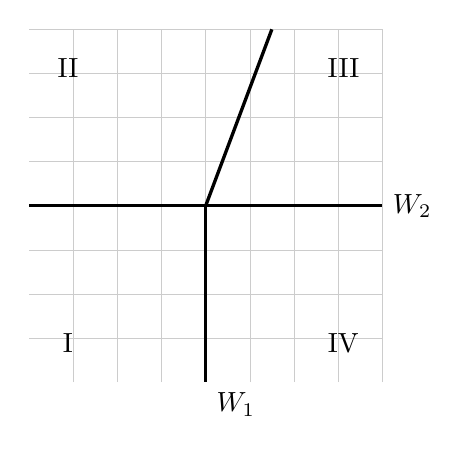
\begin{tikzpicture}[scale=0.7]

  % light square grid
  \draw[step=0.8cm,very thin,color=gray!40] (-3.2,-3.2) grid (3.2,3.2);

  % coordinate axes = walls
  \draw[very thick] (-3.2,0) -- (3.2,0) node[right] {$W_2$};
  \draw[very thick] (0,0) -- (0,-3.2) node[below right] {$W_1$};

  % slanted wall (ray) in quadrant III
  \draw[very thick] (0,0) -- (1.2,3.2);

  % chamber labels
  \node at (-2.5,-2.5) {$\mathrm{I}$};
  \node at (-2.5, 2.5) {$\mathrm{II}$};
  \node at ( 2.5, 2.5) {$\mathrm{III}$};
  \node at ( 2.5,-2.5) {$\mathrm{IV}$};

\end{tikzpicture}
\end{center}

\begin{itemize}
\item Let
\[
\cV = \cO_{\P^2_x\times\P^2_y}(-2,0)\oplus
      \cO_{\P^2_x\times\P^2_y}(-1,-3),
\]
and consider $\mathrm{tot}(\cV)$ as a toric variety given as a GIT
quotient of $\A^8$ by a torus $T\cong(\C^\ast)^2$ with weight matrix
$(t, s) \mapsto (t, t, t, s, s, s, t^{-2}, t^{-1}s^{-3})$.

\item For each wall $W_i$ there is a Kirwan-Ness stratification near
$W_i$ (Table~1 in \cite{HLS}).  The least unstable stratum has fixed
locus $Z_i$ and Levi quotient $L_i$, so that the local GIT quotient for
the wall is $Z_i/L_i$.

\item One introduces a Landau–Ginzburg potential
\[
W = p f + q g \in \C[x_i,y_j,p,q]_{\deg=2},
\]
where $f$ has bidegree $(2,0)$ and $g$ has bidegree $(1,3)$, and $f$ cuts out a smooth rational curve on $\P^2_x$.
  The LG
pair $(\cV,W)$ carries a second $\C^\ast$–grading (the LG grading, "R-charge") so that the variables $p,q$ have weight
$2$ and the $x_i,y_j$ have weight $0$, so that $W$ has weight
$2$; the associated category $D^b(\cV,W)$ is equivalent to $D^b(X)$.

  The key point is that, although $Z_i/L_i$ is \emph{non–compact} as a
  usual GIT quotient, the restriction $W|_{Z_i}$ makes the LG quotient
  $(Z_i/L_i,W|_{Z_i})$ effectively compact.  Concretely:
  \begin{itemize}
  \item Near $W_1$ one has $Z_1/L_1 \cong \P^2/\C^\ast$; the LG
        category $D^b(Z_1/L_1,W|_{Z_1})$ is equivalent to
        $D^b(\P^2)$, which admits the full exceptional collection
        $\langle \cO,\cO(1),\cO(2)\rangle$.
  \item Near $W_2$ one has $Z_2/L_2 \cong \mathrm{tot}\,\cO_{\P^2}(-2)/\C^\ast$;
        the potential restricts to $pf$. Then
        $D^b(Z_2/L_2,W|_{Z_2})\simeq D^b(C)$, and for each window this is
        equivalent to $D^b(\P^1)$ with its exceptional pair
        $\langle\cO,\cO(1)\rangle$.
  \end{itemize}

\item One finds:
  \begin{itemize}
  \item the window shift across $W_1$ is a composition of spherical
        twists around the line bundles
        \[
        \cO_X(0,i),\ \cO_X(0,i+1),\ \cO_X(0,i+2),
        \]
  \item the window shift across $W_2$ is a composition of spherical
        twists around
        \[
        \cO_X(i,0),\ \cO_X(i+1,0),
        \]
  for suitable integers $i$ (depending on the chosen windows).
  \end{itemize}
\end{itemize}

Thus, in this example the abstract window-shift autoequivalences
arising from VGIT of $(\cV,W)$ are identified explicitly with
compositions of spherical twists by line bundles on the K3 surface $X$.
\end{example}
\end{document}